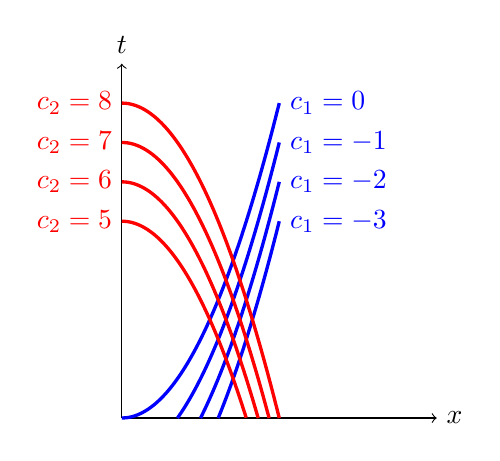
\begin{tikzpicture}
  \draw[->] (0,0) -- (4.,0) node[right] {$x$};
  \draw[->] (0,0) -- (0,4.5) node[above] {$t$};
  \draw[scale=0.5,domain=0:4,smooth,variable=\x,Blue,very thick] plot ({\x},{0.5*\x*\x}) node [right] {$c_1=0 $};
  \draw[scale=0.5,domain=1.4142:4,smooth,variable=\x,Blue,very thick] plot ({\x},{0.5*\x*\x-1}) node [right] {$c_1=-1$};
  \draw[scale=0.5,domain=2:4,smooth,variable=\x,Blue,very thick] plot ({\x},{0.5*\x*\x-2}) node [right] {$c_1=-2$};
  \draw[scale=0.5,domain=2.44948:4,smooth,variable=\x,Blue,very thick] plot ({\x},{0.5*\x*\x-3}) node [right] {$c_1=-3$};
  \draw[scale=0.5,domain=0:3.16,smooth,variable=\x,Red,very thick] plot ({\x},{-0.5*\x*\x+5});
  \node[left,Red] at (0,2.5) {$c_2=5$};
  \draw[scale=0.5,domain=0:3.4641,smooth,variable=\x,Red,very thick] plot ({\x},{-0.5*\x*\x+6});
  \node[left,Red] at (0,3) {$c_2=6$};
  \draw[scale=0.5,domain=0:3.7416,smooth,variable=\x,Red,very thick] plot ({\x},{-0.5*\x*\x+7});
  \node[left,Red] at (0,3.5) {$c_2=7$};
  \draw[scale=0.5,domain=0:4,smooth,variable=\x,Red,very thick] plot ({\x},{-0.5*\x*\x+8});
  \node[left,Red] at (0,4) {$c_2=8$};
\end{tikzpicture}
%%% Local Variables:
%%% mode: latex
%%% TeX-master: "../../mainManuscript"
%%% End:
